\label{pythonshell}
\section{Before you start}
If you're new to Python, I suggest that you first have a look at the \href{http://docs.python.org/tut/}{Python tutorial}\footnote{\url{http://docs.python.org/tut/}}. If that's not enough, abundant documentation is freely available on the \href{http://www.python.org/doc/}{Python web site}\footnote{\url{http://www.python.org/doc/}}. If you're new to stimfit, I recommend going through the tutorial in chapter \ref{gettingstarted} of this manual first.

\section{The Python shell}
When you start up stimfit, you will find an embedded Python shell in the lower part of the program window. From this shell, you have full access to the Python interpreter. For instance, you could type:
\begin{lstlisting}
>>> stf.
\end{lstlisting}
which will pop up a window showing all the available functions from the stimfit module (abbreviated \pycommand{stf}). For example, you could now check whether a file is open by selecting the \pycommand{check\_doc} \marginpy{check\_doc} function from that list: 
\begin{lstlisting}
>>> stf.check_doc()
False
\end{lstlisting} The function documentation will pop up when you type in the opening bracket. The function returns the boolean value \pycommand{False} because you haven't opened any file yet. Since the \pycommand{stf} module is imported in the namespace, you can omit the initial ``\pycommand{stf.}'' when calling functions. Thus, you could get the same result by simply typing
\begin{lstlisting}
>>> check_doc()
False
\end{lstlisting}
If you press \keybox{Ctrl} and \keybox{$\uparrow$} at the same time, you can go through all the commands that you have previously typed in. This can be very useful when you want to call a function several times in a row.

\section{Accessing data from the Python shell}
\pycommand{\textbf{get\_trace(trace=-1, channel=-1)}}\pyindex{gettrace}{get\_trace}\\
The \pycommand{get\_trace} function returns the currently displayed trace as a one-dimensional \href{http://numpy.scipy.org/}{NumPy}\footnote{\url{http://numpy.scipy.org/}} array when called without any arguments:
\begin{lstlisting}
>>> a = get_trace()
\end{lstlisting}
You can now access individual sampling points using squared brackets to specify the index. For example:
\begin{lstlisting}
>>> print a[123]
-26.3671875
\end{lstlisting}
prints out the y-value of the sampling point with index 123. Note that indices in Python are \textit{zero-based}, i.e. the first sampling point has the index 0:
\begin{lstlisting}
>>> print a[0]
-21.2249755859
\end{lstlisting}
Python will check for indices that are out of range. For example,
\begin{lstlisting}
>>> print a[1e9]
Traceback (most recent call last):
  File "<input>", line 1, in <module>
IndexError: index out of bounds
\end{lstlisting}
You can use the \pycommand{get\_trace(trace=-1, channel=-1)} function to return any trace within a file. The default values of \pycommand{trace = -1} and \pycommand{channel = -1} will return the currently displayed trace of the active channel. By passing a value of 1 as the first argument, you could access the second trace within your file (assuming it contains more than one trace, of course) - remember that indices are zero-based!
\begin{lstlisting}
>>> b = get_trace(1)
>>> print b[234]
-23.7731933594
\end{lstlisting}

\section{Using NumPy with stimfit}
\href{http://numpy.scipy.org/}{NumPy}\footnote{\url{http://numpy.scipy.org/}} allows you to efficiently perform array computations from the Python shell. For example, you can multiply an array with a scalar:
\begin{lstlisting}
>>> a = get_trace()
>>> print a[234]
-27.0385742188
>>> b = a*2
>>> print b[234]
-54.0771484375
\end{lstlisting}
Or you can multiply two arrays:
\begin{lstlisting}
>>> a = get_trace()
>>> b = get_trace(1)
>>> c = a*b
>>> print a[234], "*", b[234], "=", c[234]
-27.0385742188 * -23.7731933594 = 642.793253064
\end{lstlisting}
\pycommand{\textbf{new\_window()}}\pyindex{newwindow}{new\_window}\\
You can now display the results of the operations in a new window by passing a 1D-NumPy array to the \pycommand{new\_window} function:
\begin{lstlisting}
>>> new_window(c)
\end{lstlisting}
The sampling rate and units will be copied from the window of origin. A short way of doing all of the above within a single line would have been:
\begin{lstlisting}
>>> new_window(get_trace() * get_trace(1))
\end{lstlisting}
\pycommand{\textbf{new\_window\_matrix()}}\pyindex{newwindowmatrix}{new\_window\_matrix}\\
You can pass a 2D-NumPy array to \pycommand{new\_window\_matrix}. The first dimension will be translated into individual traces, the second dimension into sampling points. This example will put the current trace and its square root into subsequent traces of a new window:
\begin{lstlisting}
>>> numpy_matrix = N.empty( (2, get_size_trace()) )
>>> numpy_matrix[0] = get_trace()
>>> numpy_matrix[1] = N.sqrt( N.abs(get_trace()) )
>>> new_window_matrix(numpy_matrix) 
\end{lstlisting}
In this example, \pycommand{N} is the NumPy namespace. Typing \pycommand{N.} at the command prompt
will show you all available NumPy functions. \pycommand{get\_size\_trace} will be explained later on (see p. \pageref{getsizetrace}). \smallskip \\
\pycommand{\textbf{new\_window\_list()}}\pyindex{newwindowlist}{new\_window\_list}\\
Although using a 2D-NumPy array is very efficient, there are a few drawbacks: the size of the array has to be known at construction time, and all traces have to be of equal lengths. Both problems can be avoided using \pycommand{new\_window\_list}, albeit at the price of a significant performance loss. \pycommand{new\_window\_list} takes a Python list of 1D-NumPy arrays as an argument:
\begin{lstlisting}
>>> python_list = [get_trace(),]
>>> python_list.append( \
...     N.concatenate((get_trace(), get_trace())) )
>>> new_window_list(python_list)
\end{lstlisting}
Note that items in Python lists are written between \textit{squared} brackets, and that a comma is required at the end of single-item lists.

The \href{http://www.scipy.org}{SciPy}\footnote{\url{http://www.scipy.org/}} library, which is built on top of NumPy, provides a huge amount of numerical tools such as special functions, integration, ordinary differential equation sol\-vers, gradient optimization, genetic algorithms or parallel programming tools. Due to its size, it is not packaged with stimfit by default, but I highly recommend installing it for more advanced numerical analyses.

\section{Control stimfit from the Python shell}
\subsection{Cursors}
\index{cursors}Cursors can be positioned from the Python shell using one of the \pycommand{set\_[xy]\_start} or \pycommand{set\_[xy]\_end} functions, where \pycommand{[xy]} stands for one of \pycommand{peak}, \pycommand{base} or \pycommand{fit}, depending on which cursor you want to set. Correspondingly, the \pycommand{get\_[xy]\_start} or \pycommand{get\_[xy]\_end} functions can be used to retrieve the current cursor positions.\smallskip \\
\noindent
\marginpy{set\_peak\_start\\set\_base\_start\\set\_fit\_start\\set\_peak\_end\\set\_base\_end\\set\_fit\_end\\}\pyindexonly{setpeakstart}{set\_peak\_start}\pyindexonly{setbasestart}{set\_base\_start}\pyindexonly{setfitstart}{set\_fit\_start}\pycommand{\textbf{set\_[xy]\_start(pos, is\_time = False)}} and\\
\noindent
\pyindexonly{setpeakend}{set\_peak\_end}\pyindexonly{setbaseend}{set\_base\_end}\pyindexonly{setfitend}{set\_fit\_end}\pycommand{\textbf{set\_[xy]\_end(pos, is\_time = False)}} \\
take one or two arguments. \pycommand{pos} specifies the new cursor position. \pycommand{is\_time} indicates whether \pycommand{pos} is an index, i.e. in units of sampling points (\pycommand{False}, default), or in units of time (\pycommand{True}), with the trace starting at \textit{t}\,=\,0\,ms. If there was an error, such as an out-of bounds-index, these functions will return \pycommand{False}.\smallskip \\
\noindent
\marginpy{get\_peak\_start\\get\_base\_start\\get\_fit\_start\\get\_peak\_end\\get\_base\_end\\get\_fit\_end\\}\pyindexonly{getpeakstart}{get\_peak\_start}\pyindexonly{getbasestart}{get\_base\_start}\pyindexonly{getfitstart}{get\_fit\_start}\pycommand{\textbf{get\_[xy]\_start(is\_time = False)}} and\\ 
\noindent
\pyindexonly{getpeakend}{get\_peak\_end}\pyindexonly{getbaseend}{get\_base\_end}\pyindexonly{getfitend}{get\_fit\_end}\pycommand{\textbf{get\_[xy]\_end(is\_time = False)}} \\
optionally take a single argument that indicates whether the return value should be in units of sampling points (\pycommand{is\_time = False}, default) or in units of time (\pycommand{is\_time = True}). Again, traces start at \textit{t}\,=\,0\,ms. These functions will return -1 if no file is opened at the time of the function call. Indices can be converted into time values by multiplying with \pyindex{getsamplinginterval}{get\_sampling\_interval}\pycommand{get\_sampling\_interval()}. For example:
\begin{lstlisting}
>>> print "Peak start cursor index:", get_peak_start()
Peak start cursor index: 254
>>> print "corresponds to t =", get_peak_start(True), "ms"
corresponds to t = 2.54 ms
>>> print "=", get_peak_start()*get_sampling_interval(), "ms"
= 2.54 ms
>>> set_peak_start(10, True)
True
>>> print "New cursor position:", get_peak_start()
New cursor position: 1000.0
>>> print "at t=", get_peak_start(True), "ms"
at t = 10 ms
\end{lstlisting}
The peak, baseline and latency values will not be updated until you either select a new trace, press \keybox{Enter} in the main window or call \pyindex{measure}{measure}\pycommand{measure()} from the Python shell.

\subsection{Trace selection and navigation}
\pycommand{\textbf{select\_trace(trace = -1)}}\pyindex{selecttrace}{select\_trace}\\
You can select any trace within a file by passing its zero-based index to \pycommand{select\_trace}. The function will return \pycommand{False} if there was an error. The default value of -1 will select the currently displayed trace as if you had pressed \keybox{S}. If you wanted to select every fifth trace, starting with an index of 0 and ending with an index of 9 (corresponding to numbers 1 to 10 in the drop-down box), you could do:
\begin{lstlisting}
>>> for n in range(0, 10, 5): select_trace(n)
...
True
True
\end{lstlisting}
Note that the Python \pycommand{range}\pyindex{range}{range} function omits the end point.\smallskip \\
\noindent\pyindex{unselectall}{unselect\_all}\pycommand{\textbf{unselect\_all()}}\\
\noindent\pyindex{selectall}{select\_all}\pycommand{\textbf{select\_all()}}\\
\noindent\pyindex{getselectedindices}{get\_selected\_indices}\pycommand{\textbf{get\_selected\_indices()}}\\
\noindent\pyindex{newwindowselectedthis}{new\_window\_selected\textcolor{black}{$\rightarrow$}\\\hspace*{5mm}\_this}\pycommand{\textbf{new\_window\_selected\_this()}}\\
\noindent The list of selected traces can be cleared using \pycommand{unselect\_all()}, and conversely, all traces can be selected using \pycommand{select\_all()}. \pycommand{get\_selected\_indices()} returns the indices of all selected traces as a Python tuple. Finally, the selected traces within a file can be shown in a new window using \pycommand{new\_window\_selected\_this()}.\smallskip \\
\noindent\pyindex{getsizetrace}{get\_size\_trace}\pycommand{\textbf{get\_size\_trace(trace=-1, channel=-1)}} and\\
\noindent\pyindex{getsizechannel}{get\_size\_channel}\pycommand{\textbf{get\_size\_channel(channel=-1)}}\\
return the number of sampling points in a trace and the number of traces in a channel, respectively. \pycommand{trace} and \pycommand{channel} have the same meaning as in \pycommand{get\_trace} (see p. \pageref{gettrace}). These functions can be used to iterate over an entire file or to check ranges:
\begin{lstlisting}
>>> unselect_all()
>>> for n in range(0, get_size_channel(), 5): select_trace(n)
...
True
True
>>> print get_selected_indices()
(0, 5)
>>> for n in get_selected_indices():
...     print "Length of trace", n, ":", get_size_trace(n)
... 
Length of trace 0 : 13050
Length of trace 5 : 13050
\end{lstlisting}
Use backspace to remove the indentation after you have finished the second for-loop in line 10.\smallskip \\
\pycommand{\textbf{set\_trace(trace)}}\pyindex{settrace}{set\_trace}\\
sets the currently displayed trace to the specified zero-based index and returns \pycommand{False} if there was an error. This will update the peak, base and latency values, so there's no need to call \pycommand{measure()} directly after this function. \smallskip \\
\pycommand{\textbf{get\_trace\_index()}}\pyindex{gettraceindex}{get\_trace\_index}\\
Correspondingly, \pycommand{get\_trace\_index()} allows you to retrieve the zero-based index of the currently displayed trace. There is a slight inconsistency in function naming here: don't confound this function with \pycommand{get\_trace()} (see p. \pageref{gettrace}).

\subsection{File I/O}
\noindent\pyindex{fileopen}{file\_open}\pycommand{\textbf{file\_open(filename)}}\\
\noindent\pyindex{filesave}{file\_save}\pycommand{\textbf{file\_save(filename)}}\\
\noindent will open or save a file specified by \pycommand{filename}. On Windows, use double backslashes (\textbackslash\textbackslash) between directories to avoid conversion to special characters such as \textbackslash{t} or \textbackslash{n}; for example:
\begin{lstlisting}
>>> file_save("C:\\data\\datafile.dat")
\end{lstlisting}
in Windows or
\begin{lstlisting}
>>> file_save("/home/cs/data/datafile.dat")
\end{lstlisting}
in GNU/Linux. \smallskip \\
\noindent\pyindex{closethis}{close\_this}\pycommand{\textbf{close\_this()}}\\
will close the currently displayed file, whereas \smallskip \\
\noindent\pyindex{closeall}{close\_all}\pycommand{\textbf{close\_all()}}\\
closes all open files.

\subsection{Define your own functions}
By defining your own functions, you can apply identical complex analyses to different traces and files. The following steps are required to make use of your own Python files:
\begin{enumerate}
 \item Create a Python file in a directory that the Python interpreter will find. If you don't know where that is, use the stimfit program directory (typically, this will be C:{\textbackslash}Program Files{\textbackslash}Stimfit in Windows or /usr/lib/python-2.5/site-packages/\linebreak[0]stimfit in Linux). You will find some example files in that directory that you can use as a template, but you shouldn't touch stf.py which is the core stimfit module.
 \item Import the stimfit module in your file:
\begin{lstlisting}
import stf
\end{lstlisting}
\item Start stimfit and import your file in the embedded Python shell. Assuming that your file is called myFile.py, you would do:
\begin{lstlisting}
>>> import myFile
\end{lstlisting}
\item If you have applied changes to your file, there's no need to restart stimfit. Just do:
\begin{lstlisting}
>>> reload(myFile)
\end{lstlisting}
from the embedded Python shell.
\end{enumerate}
To give you an example, listing \ref{firstfile} shows a function that returns the sum of the squared amplitude values across all selected traces of a file.
\begin{listing}
\lstset{numbers=left}
\begin{lstlisting}
# import the stimfit core module:
import stf

def get_amp():
    """Returns the amplitude (peak-base)"""
    return stf.get_peak()-stf.get_base()

def sqr_amp():
    """Returns the sum of squared amplitudes of all 
    selected traces, or -1 if there was an error. Uses 
    the current settings for the peak direction and 
    cursor positions."""

    # Store the current trace index:
    old_index = stf.get_trace_index()

    sum_sqr = 0
    for n in stf.get_selected_indices():
        # Setting a trace will update all measurements,
        # so there's no need to call measure()
        if ( not(stf.set_trace(n)) ):
            return -1
        sum_sqr += get_amp()**2

    # Restore the displayed trace:
    stf.set_trace(old_index)

    return sum_sqr
\end{lstlisting}
\lstset{numbers=none}
  \caption {
    myFile.py
  }
  \label{firstfile}
\end{listing}

To import and use this file from stimfit, you would do:
\begin{lstlisting}
>>> import myFile
>>> myFile.sqr_amp()
497.70163353882447
\end{lstlisting}

\section{Some recipes for commonly requested features}
Some often-requested features could not be integrated into the program easily without cluttering up the user interface. The following sections will show how the Python shell can be used to solve these problems.

%\subsection{Multiple peak analysis}
%The peak window cursors allow to detect a single peak within the peak window. However, it may sometimes be useful to detect \keyindex{multiplepeaks}{peak!multiple peaks}{multiple peaks}multiple peaks within a trace. For instance, the recording in Fig. \ref{popspike} shows a population spike with two positive-going peaks and a negative-going peak in between.
%  \begin{myfigure}[htb]
%    \begin{center}
%      %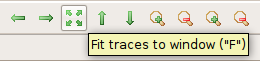
\includegraphics[scale=0.5]{./img/fittowindow.eps}
%    \end{center}
%    \caption{A population spike with multiple peaks (courtesy of Francisco Dubiela).}
%    \label{popspike}
%  \end{myfigure}
 
\subsection{Cutting traces to arbitrary lengths}
Cutting traces\keyindex{cuttingtraces}{traces!cutting}{trace cutting} is best
done using the squared bracket index operators (\pycommand{[]}) to slice a NumPy array. For example, if you wanted to cut a trace at the 100th sampling point, you could do:
\begin{lstlisting}
>>> a = get_trace()
>>> new_window(a[:100])
>>> new_window(a[100:])
\end{lstlisting}
In this example, \pycommand{a[:100]} refers to a sliced NumPy array that comprises all sampling points from index 0 to index 99, and \pycommand{a[100:]} refers to an array from index 100 to the last sampling point. \smallskip \\
\pycommand{\textbf{cut\_traces(pt)}}\pyindex{cuttraces}{cut\_traces}\\
\pycommand{\textbf{cut\_traces\_multi(pt\_list)}}\pyindex{cuttracesmulti}{cut\_traces\_multi}\\
These functions cut all selected traces at a single sampling point (\pycommand{pt}) or at multiple sampling points (\pycommand{pt\_list}). The cut traces will be shown in a new window. Both functions are included in the \pycommand{stf} namespace from version 0.8.11 on. The code for \pycommand{cut\_traces} is shown in listing \ref{cuttraceslisting}.
\begin{listing}
\lstset{numbers=left}
\begin{lstlisting}
import stf
import numpy as N

def cut_traces( pt ):
    """Cuts the selected traces at the sampling point pt,
    and shows the cut traces in a new window.
    Returns True upon success, False upon failure."""

    # Check whether anything has been selected:
    if not stf.get_selected_indices():
        return False
    new_list = list()
    for n in stf.get_selected_indices():
        if not stf.set_trace(n): return False

        # Check for out of range:
        if pt < stf.get_size_trace():
            new_list.append( stf.get_trace()[:pt] )
            new_list.append( stf.get_trace()[pt:] )
        else:
            print "Cutting point", pt, "is out of range"

    # Don't create a new window if everything was out of
    # range
    if len(new_list) > 0: stf.new_window_list( new_list )

    return True
\end{lstlisting}
\lstset{numbers=none}
  \caption {
    \pycommand{cut\_traces}
  }
  \label{cuttraceslisting}
\end{listing}
For example,
\begin{lstlisting}
>>> cut_traces_multi([100,900])
\end{lstlisting}
will cut all selected traces at sampling points 100 and 900 and show the cut traces in a new window. Note that you can pass a list or a tuple as an argument.
\begin{lstlisting}
>>> cut_traces_multi(range(100,2000,100))
\end{lstlisting}
will cut the selected traces at every 100th sampling point, starting with the 100th and ending with the 1900th (see p. \pageref{range} for the syntax of the \pycommand{range} function).
